% Problem 3 -- included from hw.tex via % Problem 3 -- included from hw.tex via % Problem 3 -- included from hw.tex via % Problem 3 -- included from hw.tex via \input{problems/problem3}.
% Paths (figures/, *.py) are relative to the directory of hw.tex.

%===============================================================================
\section*{Problem 3: Backward Reachable Set -- Programming}
%===============================================================================

\subsection*{Implementation}

The robot advances one row per step and can shift by at most one column,
$(x_{\tvar+1},y_{\tvar+1})=(x_\tvar+\ctrl_\tvar,\,y_\tvar+1)$ with $\ctrl_\tvar\in\{-1,0,1\}$;
landing on an obstacle cell is a failure. \lstinline{get_successors} returns the cells reachable in
one step (moves that would leave the grid are treated as inadmissible; for the obstacle layout in
this problem the tube never touches the side walls, so this choice does not affect the results).
\lstinline{calculate_inevitable_brt} computes the inevitable BRT of the failure set $\failure$ by
the fixed-point iteration
\[
\inevitable{\backward{\reach}}_{0}=\failure,\qquad
\inevitable{\backward{\reach}}_{k+1}=\inevitable{\backward{\reach}}_{k}\ \cup\
\bigl\{\state:\ \dyn(\state,\ctrl)\in\inevitable{\backward{\reach}}_{k}\ \text{for \emph{all}}\ \ctrl\in\{-1,0,1\}\bigr\},
\]
i.e.\ a cell is added when every admissible control leads into the current set (no escape route),
and the iteration stops when a sweep adds nothing. Because $y$ increases by one every step, only the
rows below the highest obstacle row can ever collide, and the loop converges after at most that many
sweeps. The complement of the resulting set is the (all-time) safe set $\safeset(\failure)$; this is
the discrete-time, finite-state counterpart of the HJ reachability formulation
in~\cite{bansal2017hamilton}.

\lstinputlisting[language=Python]{get_successors.py}
\lstinputlisting[language=Python]{calculate_inevitable_brt.py}

\subsection*{Results}

\noindent\begin{minipage}{\linewidth}
Figure~\ref{fig:brt} shows the grid world and the three inevitable BRTs produced by the notebook.
With obstacle~1 occupying columns $\{2,3,4\}$ of row~5 and obstacle~2 occupying columns $\{5,6\}$:
\begin{center}
\begin{tabular}{ll}
\hline
failure set & inevitable BRT minus the obstacle cells \\
\hline
obstacle 1 (width 3) & $\{(3,4)\}$ \\
obstacle 2 (width 2) & $\emptyset$ \\
both obstacles (width 5) & $\{(3,4),(4,4),(5,4),(4,3)\}$ \\
\hline
\end{tabular}
\end{center}
\end{minipage}

\begin{figure}[h]
\centering
\begin{subfigure}[t]{0.42\linewidth}
  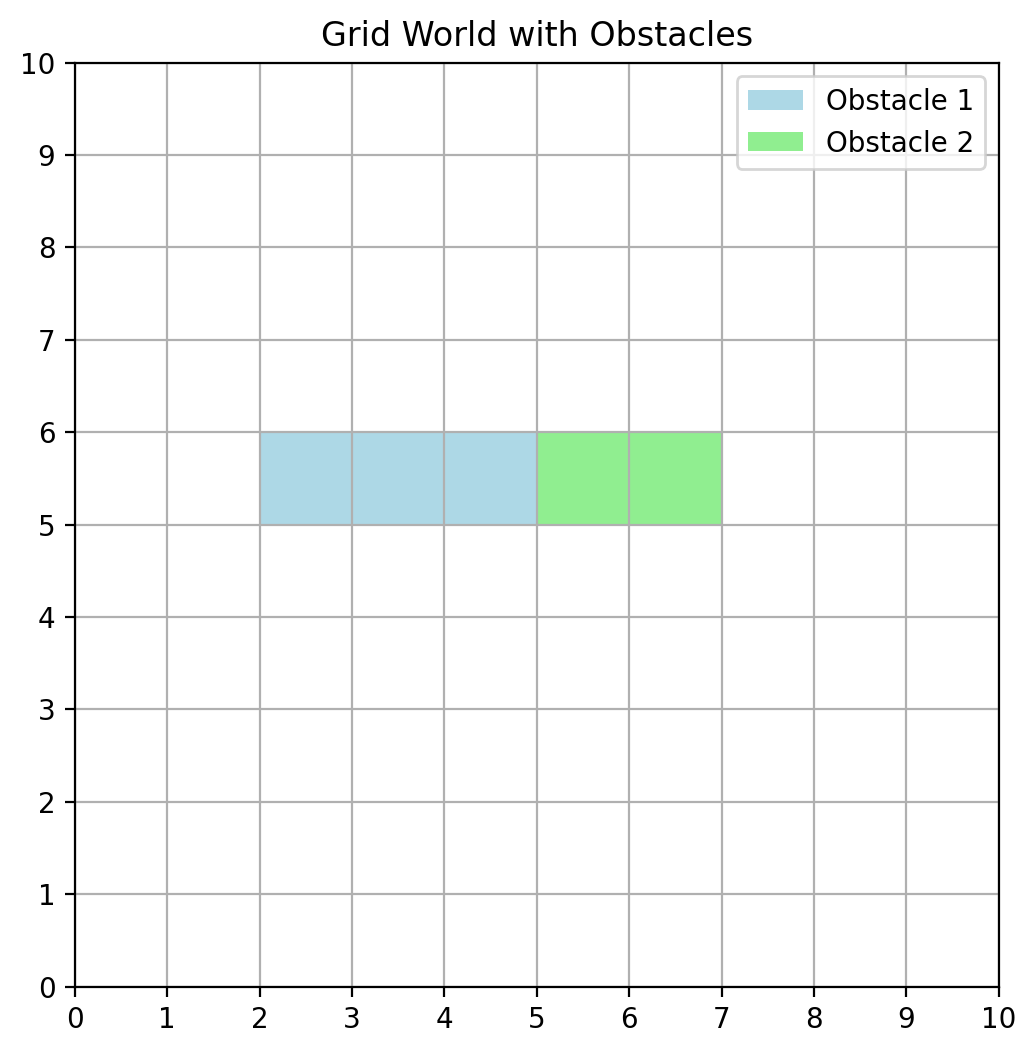
\includegraphics[width=\linewidth]{figures/world.png}
  \caption{The grid world.}
\end{subfigure}\hfill
\begin{subfigure}[t]{0.42\linewidth}
  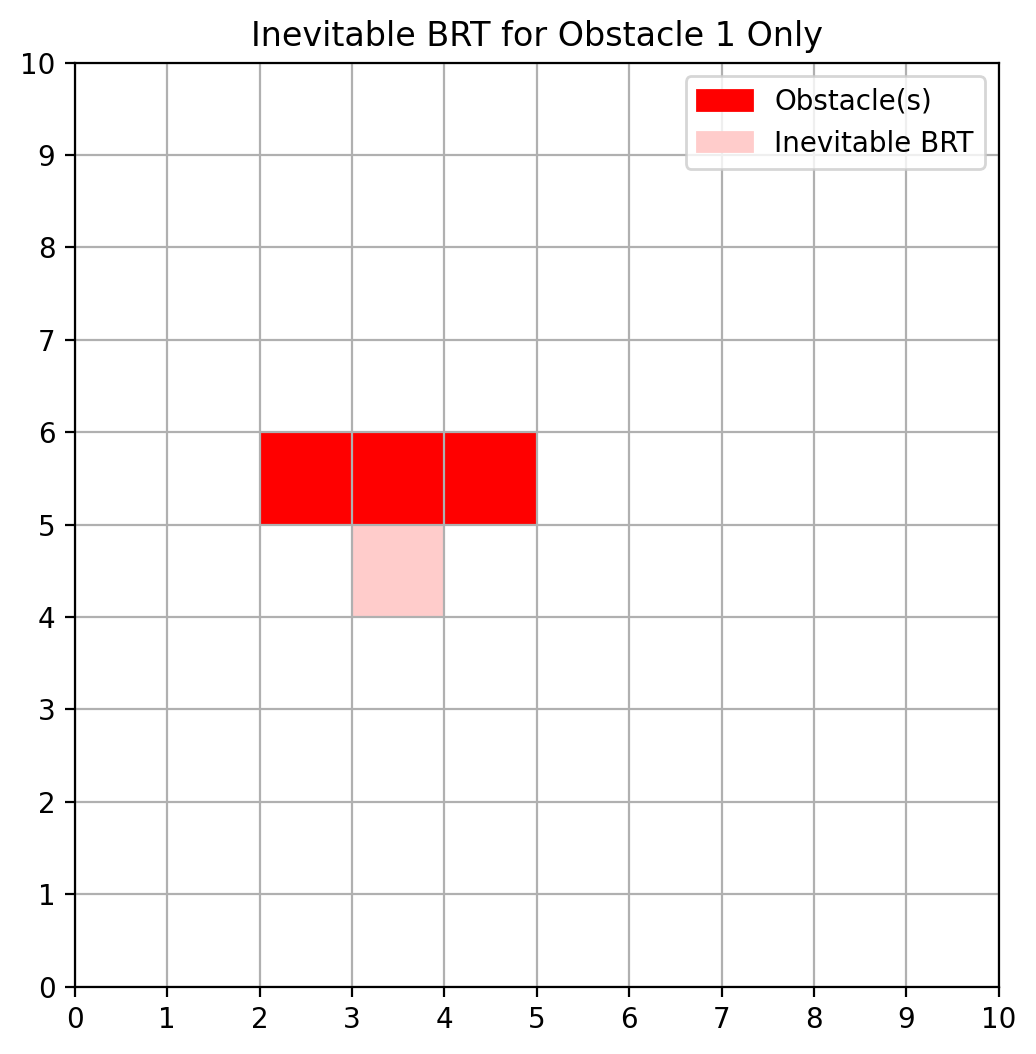
\includegraphics[width=\linewidth]{figures/brt_obstacle1.png}
  \caption{Obstacle 1 only.}
\end{subfigure}\\[2mm]
\begin{subfigure}[t]{0.42\linewidth}
  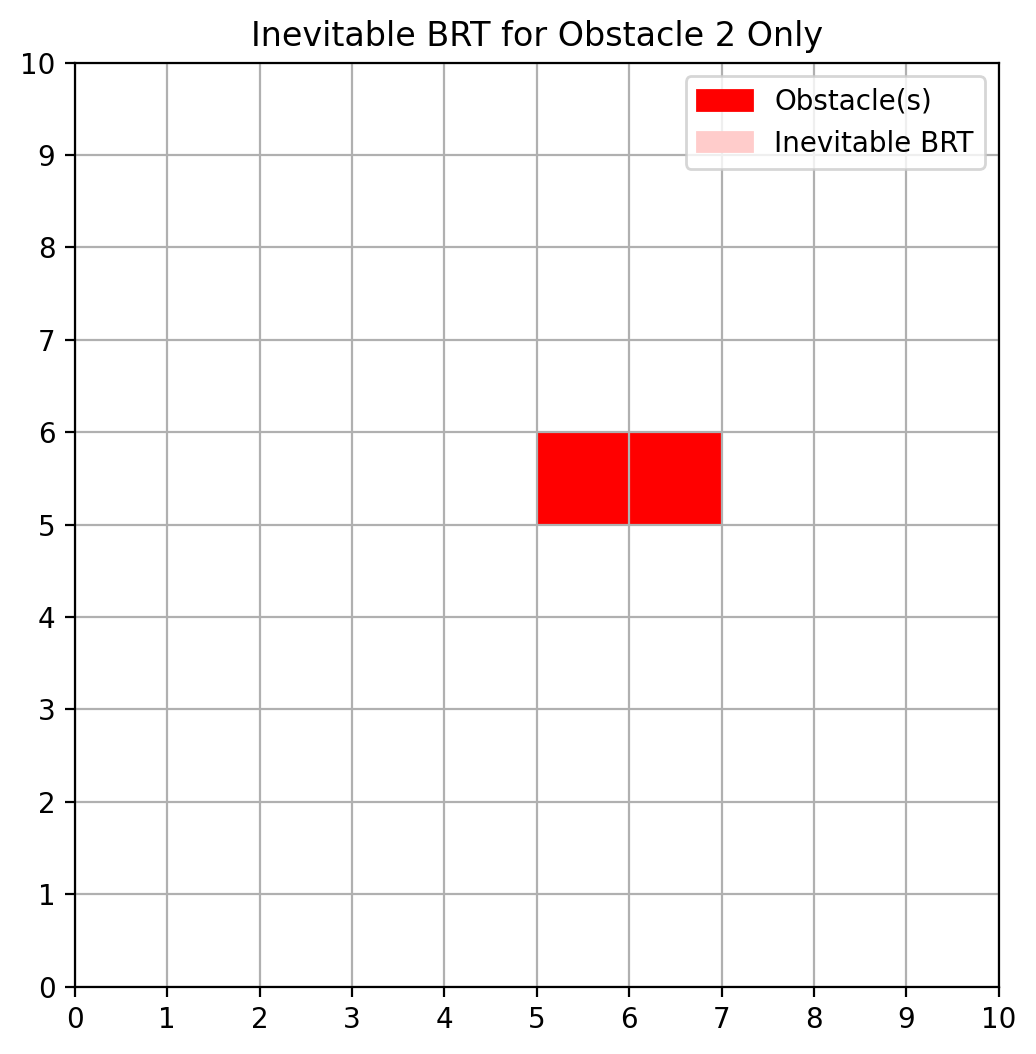
\includegraphics[width=\linewidth]{figures/brt_obstacle2.png}
  \caption{Obstacle 2 only.}
\end{subfigure}\hfill
\begin{subfigure}[t]{0.42\linewidth}
  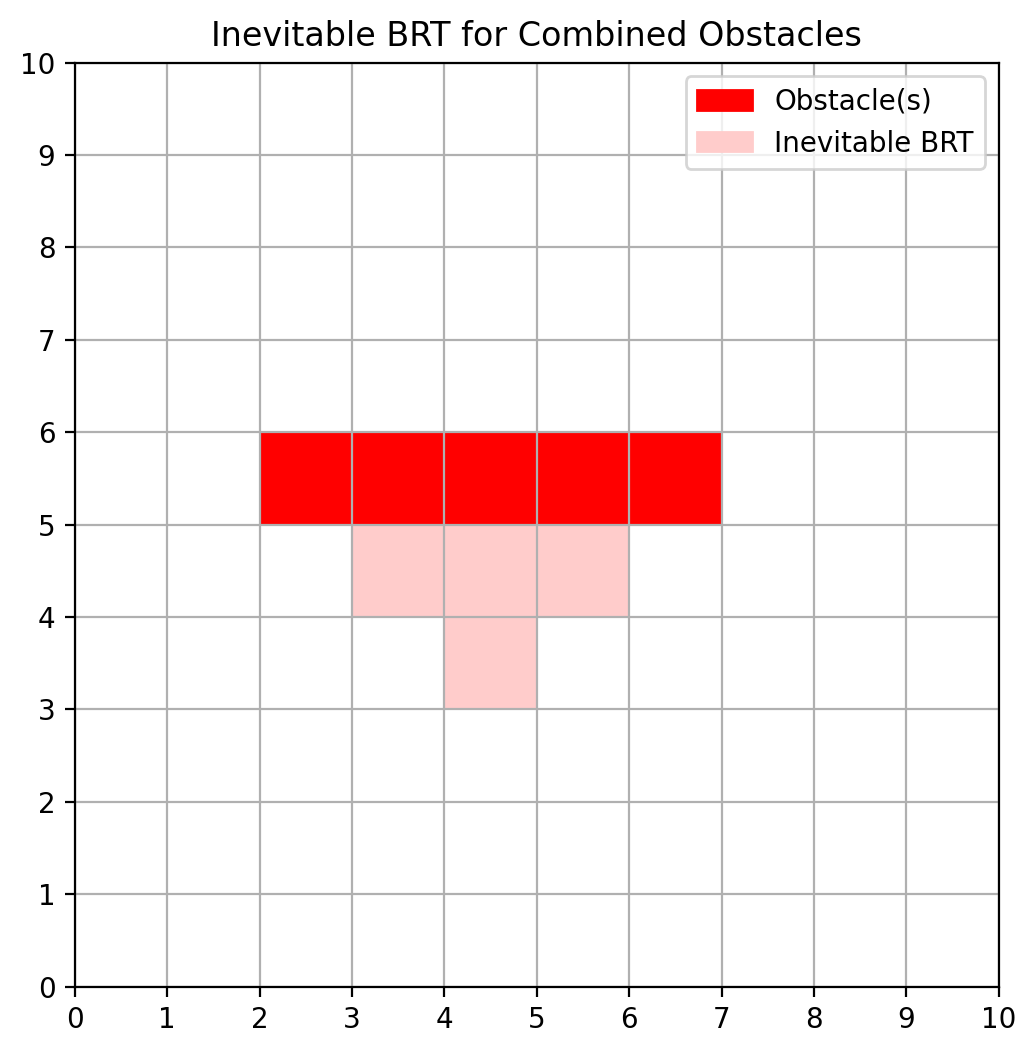
\includegraphics[width=\linewidth]{figures/brt_combined.png}
  \caption{Both obstacles.}
\end{subfigure}
\caption{Inevitable backward-reachable tubes (light red) of the obstacle sets (red).}
\label{fig:brt}
\end{figure}

\subsection*{Discussion}

\paragraph{Why the tubes look the way they do.}
The robot cannot stop or slow down, so a cell $d$ rows below the obstacle row will land on that row
after exactly $d$ steps, at a column anywhere in $\{x-d,\dots,x+d\}$ (any integer in that range is
attainable by an appropriate control sequence). Collision is inevitable if and only if
\emph{every} one of those landing columns is occupied, i.e.\ $\{x-d,\dots,x+d\}\subseteq$ obstacle
columns. For a contiguous obstacle of width $w$ this means $2d\le w-1$, so the tube is an inverted
triangle (a cone with unit slope) of height $\lfloor (w-1)/2\rfloor$ below the obstacle's centre:
height $1$ for the width-3 obstacle, height $0$ for the width-2 obstacle, and height $2$ for the
combined width-5 obstacle. This is exactly what the code produces, and it matches intuition: since
the robot's lateral speed equals its forward speed, it can escape any obstacle whose half-width is
smaller than its current distance to the obstacle row, so the doomed region hugs the obstacle
tightly. Everything above the obstacle row and everything in the rows below it that is outside the
cone is safe. Note that the width-2 obstacle alone has an empty tube beyond itself: from $(5,4)$ or
$(6,4)$ the robot can always step to a free neighbouring column.

\paragraph{Combined obstacles versus the union of the individual tubes.}
The union of the two individual tubes adds only $(3,4)$ to the obstacle cells, whereas the tube of
the combined failure set adds $(3,4)$, $(4,4)$, $(5,4)$ and $(4,3)$ (Figure~\ref{fig:union}). The
combined tube \emph{strictly contains} the union. The extra cells are states from which every escape
from one obstacle lands in the other: from $(4,4)$, steering left or going straight hits obstacle~1
while steering right hits obstacle~2, and from $(4,3)$ all three successors are among these doomed
cells. This is the discrete version of Problem~1.2(c): a state can be safe with respect to
$\failure_1$ and safe with respect to $\failure_2$ using two \emph{different} controllers, yet unsafe
with respect to $\failure_1\cup\failure_2$, i.e.\
$\safeset(\failure_1\cup\failure_2)\subsetneq\safeset(\failure_1)\cap\safeset(\failure_2)$ and,
equivalently, $\inevitable{\backward{\reach}}(\failure_1\cup\failure_2)\supsetneq
\inevitable{\backward{\reach}}(\failure_1)\cup\inevitable{\backward{\reach}}(\failure_2)$. The
practical lesson is that safety analysis must be carried out on the \emph{full} failure set;
per-obstacle tubes cannot simply be unioned, and a ``harmless'' obstacle (obstacle~2 alone traps
nothing) can enlarge the unsafe region substantially once it sits next to another one. The boundary
of the tube is also where a least-restrictive safety filter would have to intervene: from $(3,3)$
the only safe action is $\ctrl=-1$, so the filter must override $\ctrl\in\{0,+1\}$ there, while it
can leave the controller free anywhere outside the tube.

\begin{figure}[h]
\centering
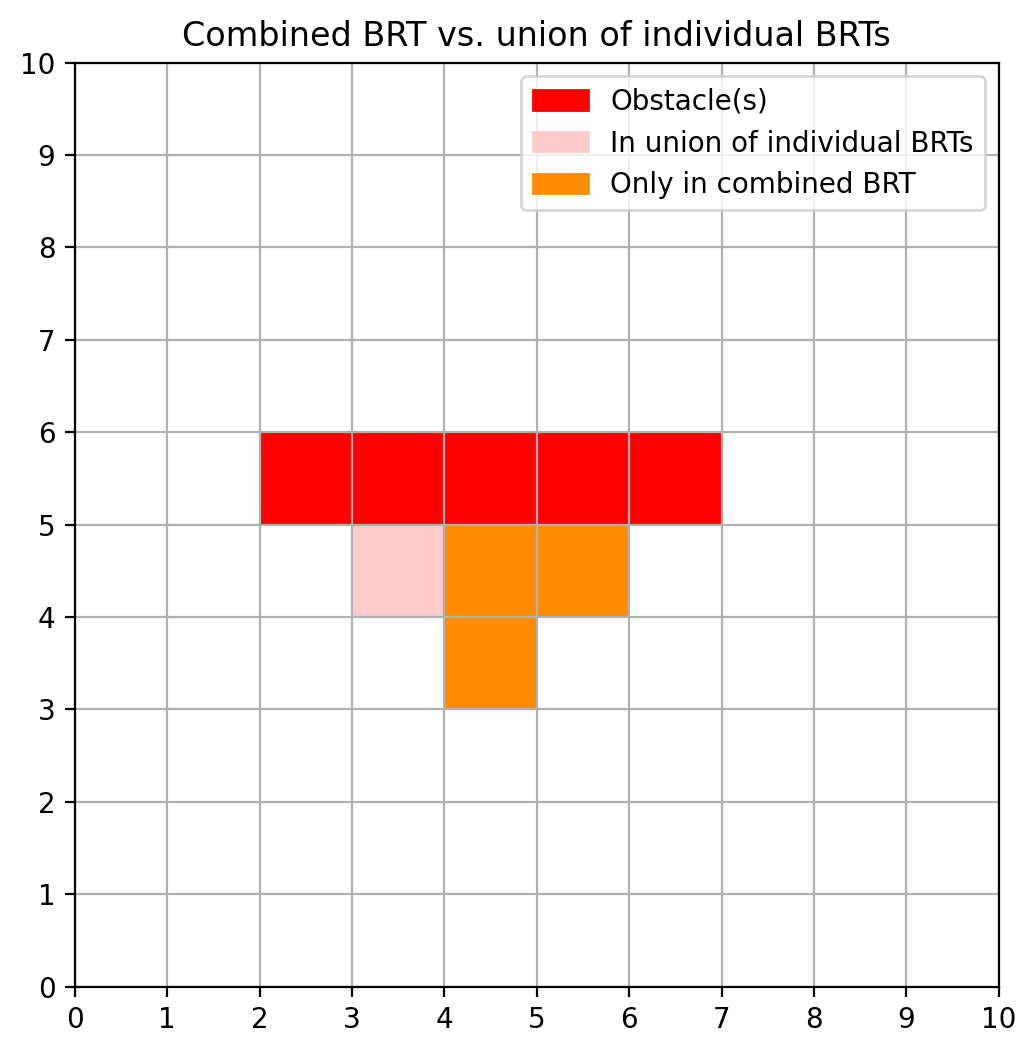
\includegraphics[width=0.42\linewidth]{figures/brt_union_vs_combined.png}
\caption{The tube of the combined failure set. Light red cells also belong to the union of the two
individual tubes; orange cells belong only to the combined tube.}
\label{fig:union}
\end{figure}

\paragraph{Effect of the forward-to-lateral speed ratio.}
The shape of the tube is set by the ratio of lateral to forward speed. If the robot advanced $v$
rows per step while still shifting by at most one column (equivalently, it could steer only once
every $v$ rows), then from $d$ rows away it could only reach columns within $\pm d/v$ of its current
one, and the trapping condition becomes $2d/v\le w-1$: the cone becomes steeper and its height grows
to about $v(w-1)/2$, so the inevitable tube \emph{grows}. A faster robot has fewer steps in which to
swerve, and in the limit of very fast forward motion every cell in the obstacle's ``shadow''
directly below it becomes doomed. Conversely, more lateral authority ($\ctrl\in\{-k,\dots,k\}$)
flattens the cone to height $\lfloor (w-1)/(2k)\rfloor$; with $k=2$ the combined tube would shrink to
the obstacles plus the single cell $(4,4)$, and obstacle~1's tube would shrink to the obstacle itself.
(In the literal discrete model a speed of $v=2$ rows per step also introduces a parity effect: a
robot starting on an even row would hop over the single obstacle row entirely, since grazing is
allowed. The statement above should therefore be read in the fine-grid or continuous-time limit,
where the obstacle has finite thickness.)
.
% Paths (figures/, *.py) are relative to the directory of hw.tex.

%===============================================================================
\section*{Problem 3: Backward Reachable Set -- Programming}
%===============================================================================

\subsection*{Implementation}

The robot advances one row per step and can shift by at most one column,
$(x_{\tvar+1},y_{\tvar+1})=(x_\tvar+\ctrl_\tvar,\,y_\tvar+1)$ with $\ctrl_\tvar\in\{-1,0,1\}$;
landing on an obstacle cell is a failure. \lstinline{get_successors} returns the cells reachable in
one step (moves that would leave the grid are treated as inadmissible; for the obstacle layout in
this problem the tube never touches the side walls, so this choice does not affect the results).
\lstinline{calculate_inevitable_brt} computes the inevitable BRT of the failure set $\failure$ by
the fixed-point iteration
\[
\inevitable{\backward{\reach}}_{0}=\failure,\qquad
\inevitable{\backward{\reach}}_{k+1}=\inevitable{\backward{\reach}}_{k}\ \cup\
\bigl\{\state:\ \dyn(\state,\ctrl)\in\inevitable{\backward{\reach}}_{k}\ \text{for \emph{all}}\ \ctrl\in\{-1,0,1\}\bigr\},
\]
i.e.\ a cell is added when every admissible control leads into the current set (no escape route),
and the iteration stops when a sweep adds nothing. Because $y$ increases by one every step, only the
rows below the highest obstacle row can ever collide, and the loop converges after at most that many
sweeps. The complement of the resulting set is the (all-time) safe set $\safeset(\failure)$; this is
the discrete-time, finite-state counterpart of the HJ reachability formulation
in~\cite{bansal2017hamilton}.

\lstinputlisting[language=Python]{get_successors.py}
\lstinputlisting[language=Python]{calculate_inevitable_brt.py}

\subsection*{Results}

\noindent\begin{minipage}{\linewidth}
Figure~\ref{fig:brt} shows the grid world and the three inevitable BRTs produced by the notebook.
With obstacle~1 occupying columns $\{2,3,4\}$ of row~5 and obstacle~2 occupying columns $\{5,6\}$:
\begin{center}
\begin{tabular}{ll}
\hline
failure set & inevitable BRT minus the obstacle cells \\
\hline
obstacle 1 (width 3) & $\{(3,4)\}$ \\
obstacle 2 (width 2) & $\emptyset$ \\
both obstacles (width 5) & $\{(3,4),(4,4),(5,4),(4,3)\}$ \\
\hline
\end{tabular}
\end{center}
\end{minipage}

\begin{figure}[h]
\centering
\begin{subfigure}[t]{0.42\linewidth}
  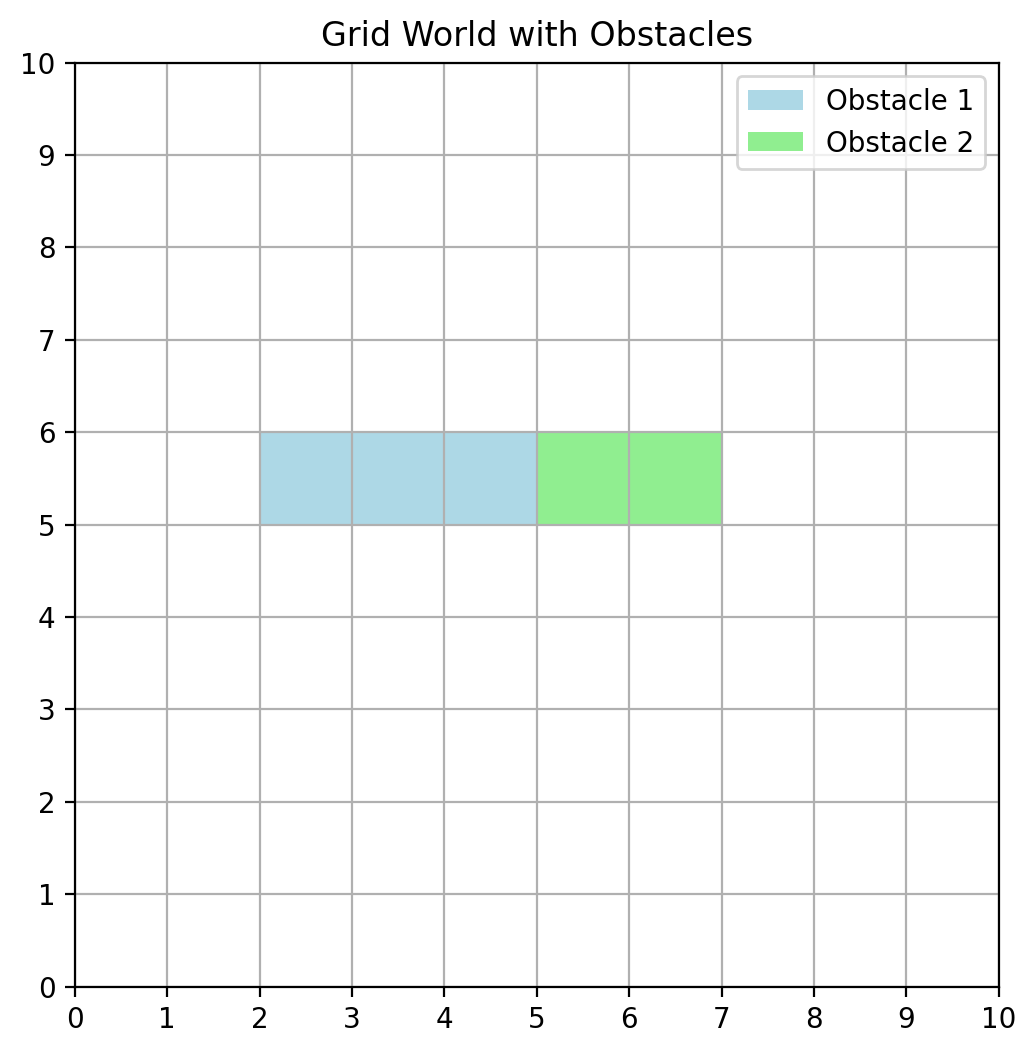
\includegraphics[width=\linewidth]{figures/world.png}
  \caption{The grid world.}
\end{subfigure}\hfill
\begin{subfigure}[t]{0.42\linewidth}
  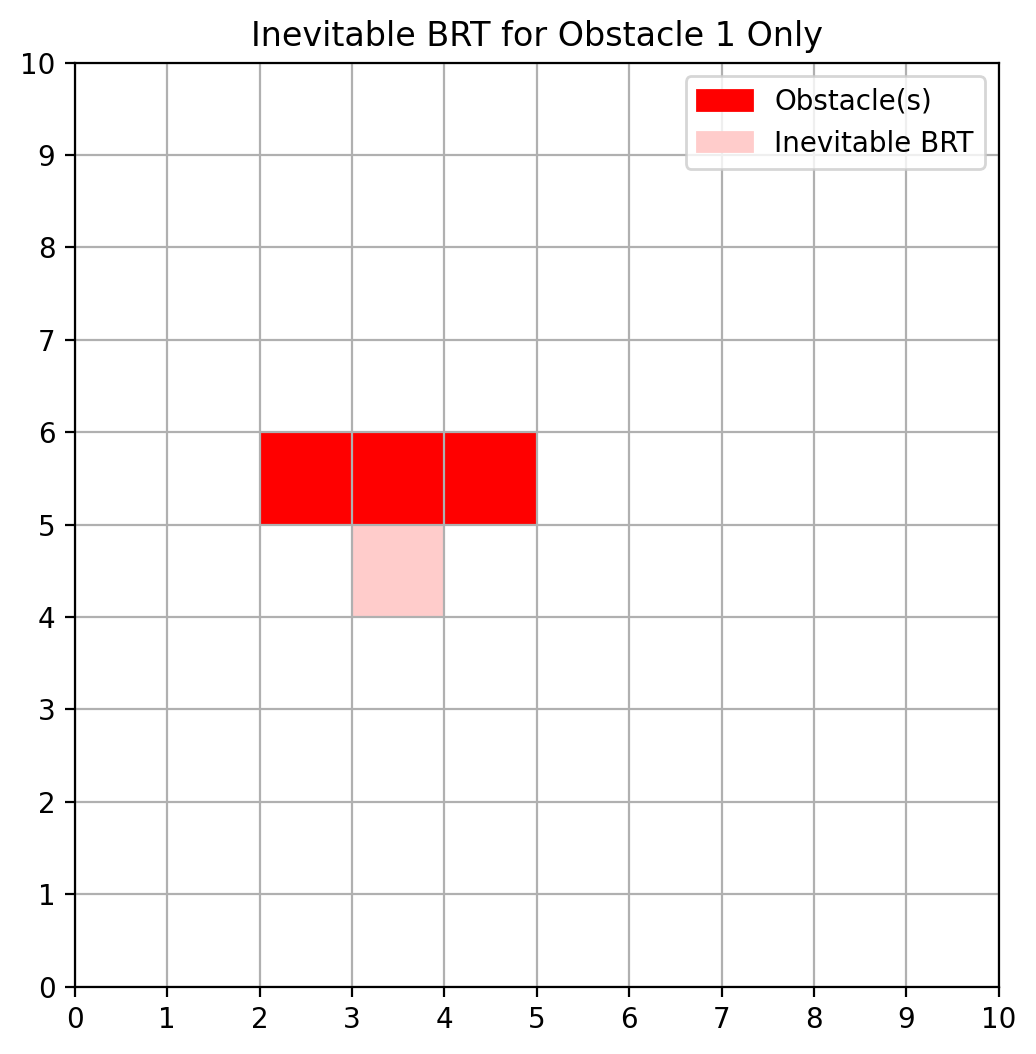
\includegraphics[width=\linewidth]{figures/brt_obstacle1.png}
  \caption{Obstacle 1 only.}
\end{subfigure}\\[2mm]
\begin{subfigure}[t]{0.42\linewidth}
  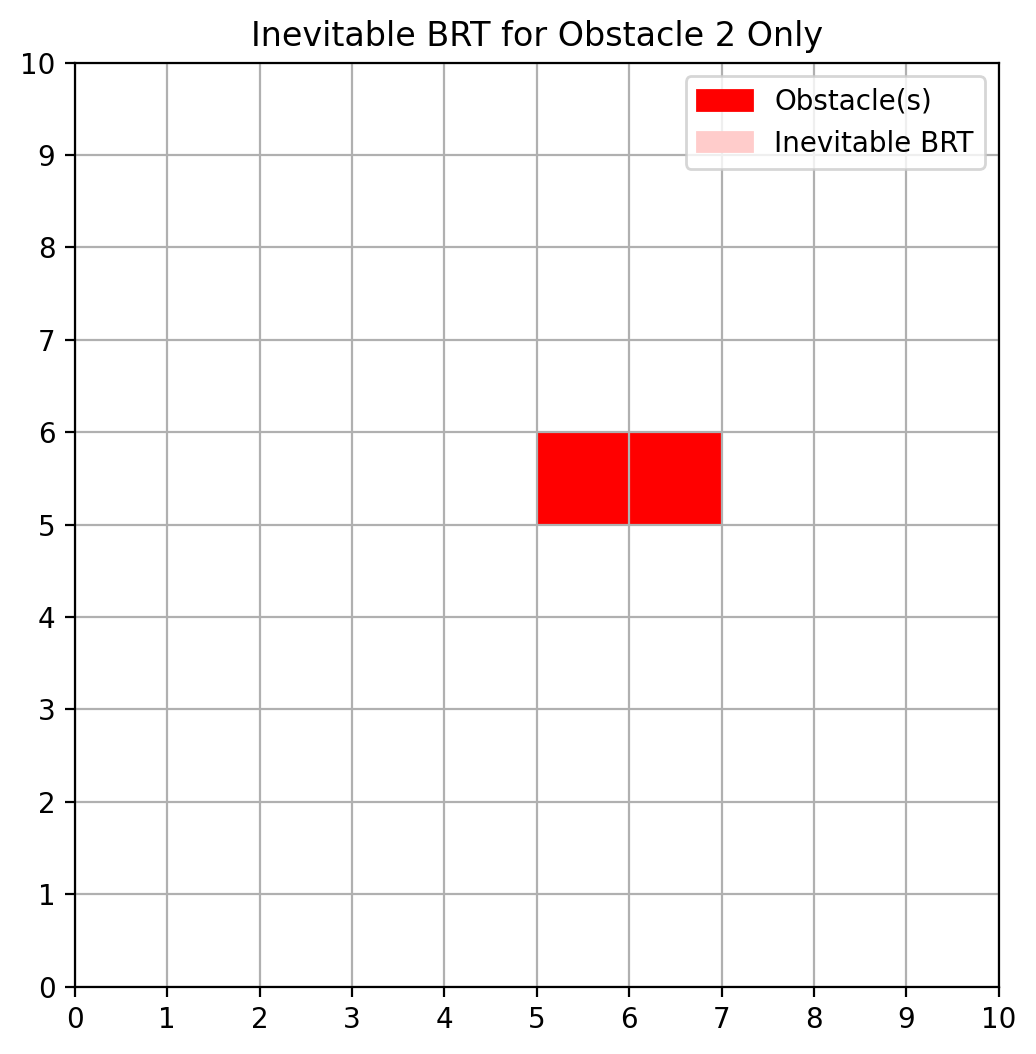
\includegraphics[width=\linewidth]{figures/brt_obstacle2.png}
  \caption{Obstacle 2 only.}
\end{subfigure}\hfill
\begin{subfigure}[t]{0.42\linewidth}
  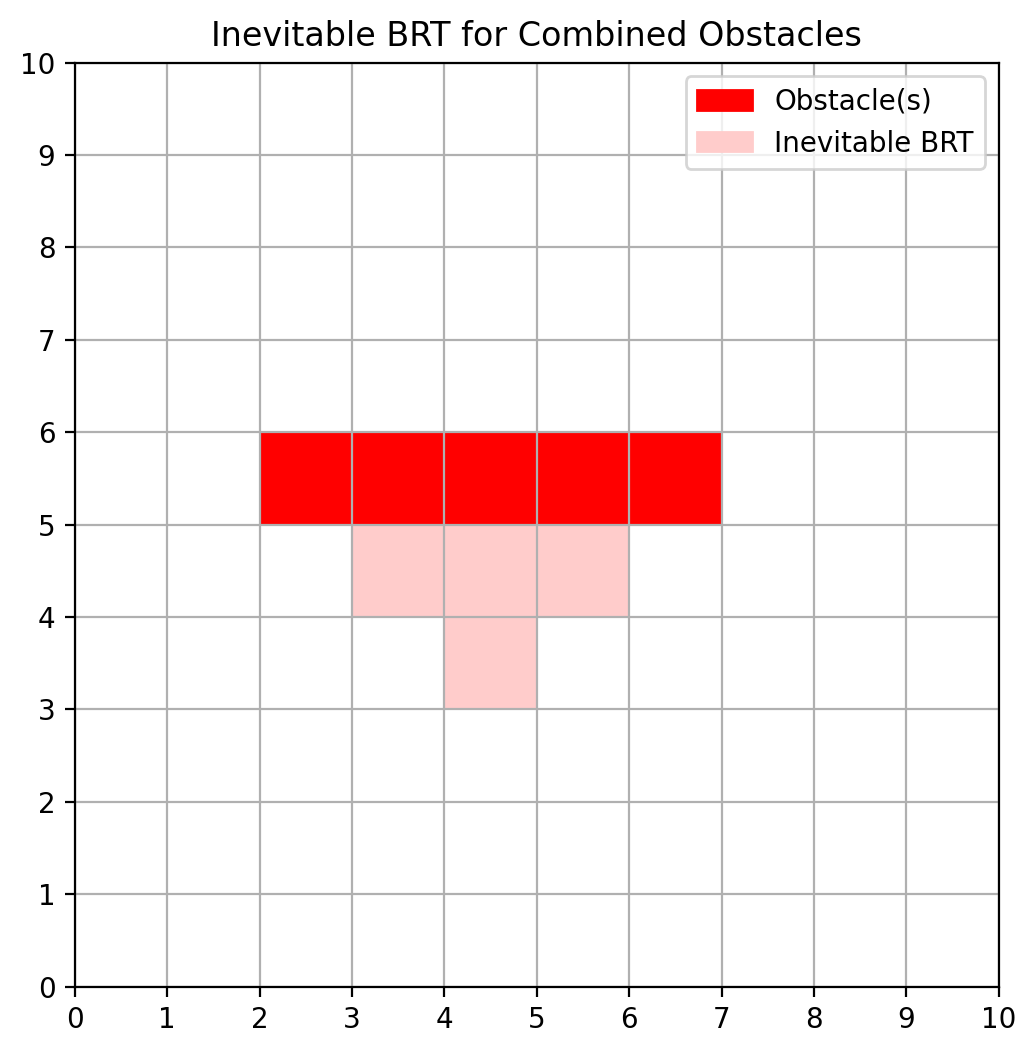
\includegraphics[width=\linewidth]{figures/brt_combined.png}
  \caption{Both obstacles.}
\end{subfigure}
\caption{Inevitable backward-reachable tubes (light red) of the obstacle sets (red).}
\label{fig:brt}
\end{figure}

\subsection*{Discussion}

\paragraph{Why the tubes look the way they do.}
The robot cannot stop or slow down, so a cell $d$ rows below the obstacle row will land on that row
after exactly $d$ steps, at a column anywhere in $\{x-d,\dots,x+d\}$ (any integer in that range is
attainable by an appropriate control sequence). Collision is inevitable if and only if
\emph{every} one of those landing columns is occupied, i.e.\ $\{x-d,\dots,x+d\}\subseteq$ obstacle
columns. For a contiguous obstacle of width $w$ this means $2d\le w-1$, so the tube is an inverted
triangle (a cone with unit slope) of height $\lfloor (w-1)/2\rfloor$ below the obstacle's centre:
height $1$ for the width-3 obstacle, height $0$ for the width-2 obstacle, and height $2$ for the
combined width-5 obstacle. This is exactly what the code produces, and it matches intuition: since
the robot's lateral speed equals its forward speed, it can escape any obstacle whose half-width is
smaller than its current distance to the obstacle row, so the doomed region hugs the obstacle
tightly. Everything above the obstacle row and everything in the rows below it that is outside the
cone is safe. Note that the width-2 obstacle alone has an empty tube beyond itself: from $(5,4)$ or
$(6,4)$ the robot can always step to a free neighbouring column.

\paragraph{Combined obstacles versus the union of the individual tubes.}
The union of the two individual tubes adds only $(3,4)$ to the obstacle cells, whereas the tube of
the combined failure set adds $(3,4)$, $(4,4)$, $(5,4)$ and $(4,3)$ (Figure~\ref{fig:union}). The
combined tube \emph{strictly contains} the union. The extra cells are states from which every escape
from one obstacle lands in the other: from $(4,4)$, steering left or going straight hits obstacle~1
while steering right hits obstacle~2, and from $(4,3)$ all three successors are among these doomed
cells. This is the discrete version of Problem~1.2(c): a state can be safe with respect to
$\failure_1$ and safe with respect to $\failure_2$ using two \emph{different} controllers, yet unsafe
with respect to $\failure_1\cup\failure_2$, i.e.\
$\safeset(\failure_1\cup\failure_2)\subsetneq\safeset(\failure_1)\cap\safeset(\failure_2)$ and,
equivalently, $\inevitable{\backward{\reach}}(\failure_1\cup\failure_2)\supsetneq
\inevitable{\backward{\reach}}(\failure_1)\cup\inevitable{\backward{\reach}}(\failure_2)$. The
practical lesson is that safety analysis must be carried out on the \emph{full} failure set;
per-obstacle tubes cannot simply be unioned, and a ``harmless'' obstacle (obstacle~2 alone traps
nothing) can enlarge the unsafe region substantially once it sits next to another one. The boundary
of the tube is also where a least-restrictive safety filter would have to intervene: from $(3,3)$
the only safe action is $\ctrl=-1$, so the filter must override $\ctrl\in\{0,+1\}$ there, while it
can leave the controller free anywhere outside the tube.

\begin{figure}[h]
\centering
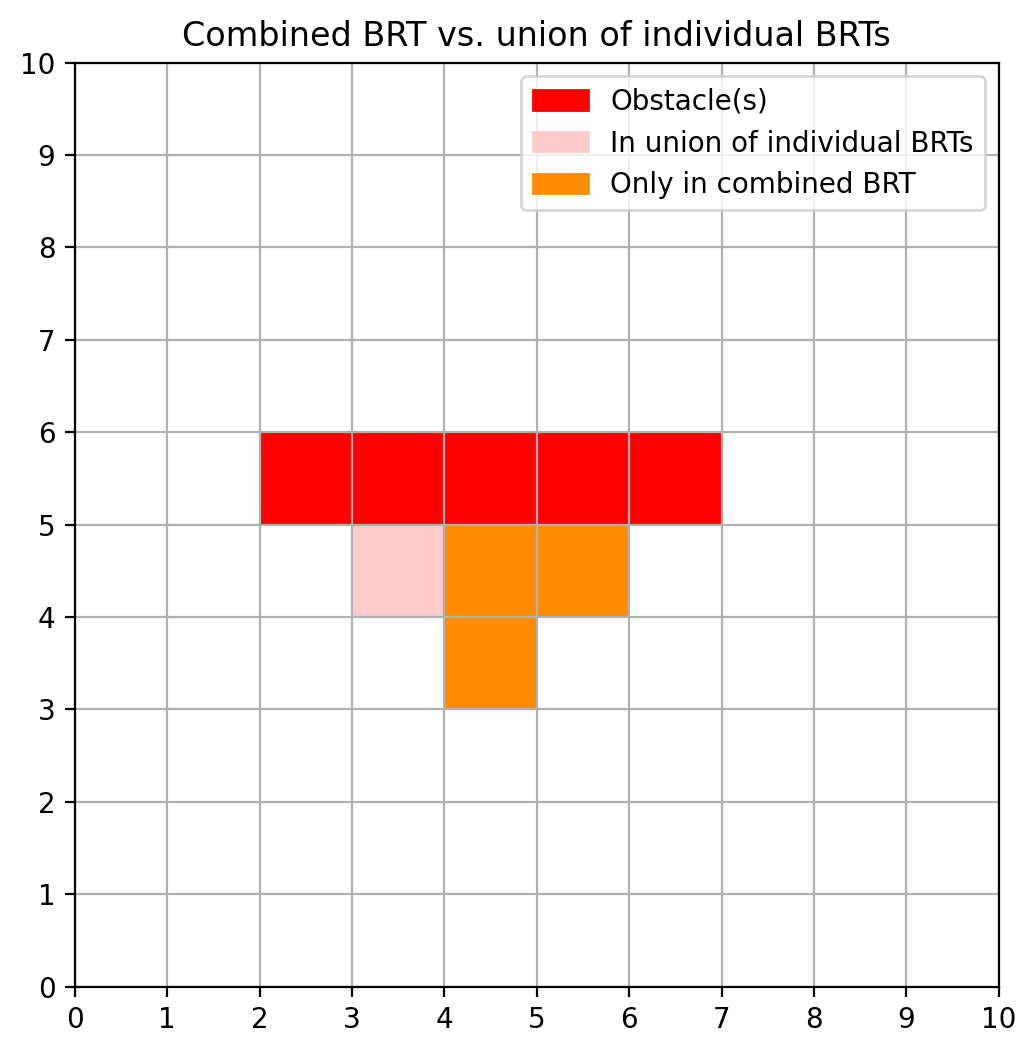
\includegraphics[width=0.42\linewidth]{figures/brt_union_vs_combined.png}
\caption{The tube of the combined failure set. Light red cells also belong to the union of the two
individual tubes; orange cells belong only to the combined tube.}
\label{fig:union}
\end{figure}

\paragraph{Effect of the forward-to-lateral speed ratio.}
The shape of the tube is set by the ratio of lateral to forward speed. If the robot advanced $v$
rows per step while still shifting by at most one column (equivalently, it could steer only once
every $v$ rows), then from $d$ rows away it could only reach columns within $\pm d/v$ of its current
one, and the trapping condition becomes $2d/v\le w-1$: the cone becomes steeper and its height grows
to about $v(w-1)/2$, so the inevitable tube \emph{grows}. A faster robot has fewer steps in which to
swerve, and in the limit of very fast forward motion every cell in the obstacle's ``shadow''
directly below it becomes doomed. Conversely, more lateral authority ($\ctrl\in\{-k,\dots,k\}$)
flattens the cone to height $\lfloor (w-1)/(2k)\rfloor$; with $k=2$ the combined tube would shrink to
the obstacles plus the single cell $(4,4)$, and obstacle~1's tube would shrink to the obstacle itself.
(In the literal discrete model a speed of $v=2$ rows per step also introduces a parity effect: a
robot starting on an even row would hop over the single obstacle row entirely, since grazing is
allowed. The statement above should therefore be read in the fine-grid or continuous-time limit,
where the obstacle has finite thickness.)
.
% Paths (figures/, *.py) are relative to the directory of hw.tex.

%===============================================================================
\section*{Problem 3: Backward Reachable Set -- Programming}
%===============================================================================

\subsection*{Implementation}

The robot advances one row per step and can shift by at most one column,
$(x_{\tvar+1},y_{\tvar+1})=(x_\tvar+\ctrl_\tvar,\,y_\tvar+1)$ with $\ctrl_\tvar\in\{-1,0,1\}$;
landing on an obstacle cell is a failure. \lstinline{get_successors} returns the cells reachable in
one step (moves that would leave the grid are treated as inadmissible; for the obstacle layout in
this problem the tube never touches the side walls, so this choice does not affect the results).
\lstinline{calculate_inevitable_brt} computes the inevitable BRT of the failure set $\failure$ by
the fixed-point iteration
\[
\inevitable{\backward{\reach}}_{0}=\failure,\qquad
\inevitable{\backward{\reach}}_{k+1}=\inevitable{\backward{\reach}}_{k}\ \cup\
\bigl\{\state:\ \dyn(\state,\ctrl)\in\inevitable{\backward{\reach}}_{k}\ \text{for \emph{all}}\ \ctrl\in\{-1,0,1\}\bigr\},
\]
i.e.\ a cell is added when every admissible control leads into the current set (no escape route),
and the iteration stops when a sweep adds nothing. Because $y$ increases by one every step, only the
rows below the highest obstacle row can ever collide, and the loop converges after at most that many
sweeps. The complement of the resulting set is the (all-time) safe set $\safeset(\failure)$; this is
the discrete-time, finite-state counterpart of the HJ reachability formulation
in~\cite{bansal2017hamilton}.

\lstinputlisting[language=Python]{get_successors.py}
\lstinputlisting[language=Python]{calculate_inevitable_brt.py}

\subsection*{Results}

\noindent\begin{minipage}{\linewidth}
Figure~\ref{fig:brt} shows the grid world and the three inevitable BRTs produced by the notebook.
With obstacle~1 occupying columns $\{2,3,4\}$ of row~5 and obstacle~2 occupying columns $\{5,6\}$:
\begin{center}
\begin{tabular}{ll}
\hline
failure set & inevitable BRT minus the obstacle cells \\
\hline
obstacle 1 (width 3) & $\{(3,4)\}$ \\
obstacle 2 (width 2) & $\emptyset$ \\
both obstacles (width 5) & $\{(3,4),(4,4),(5,4),(4,3)\}$ \\
\hline
\end{tabular}
\end{center}
\end{minipage}

\begin{figure}[h]
\centering
\begin{subfigure}[t]{0.42\linewidth}
  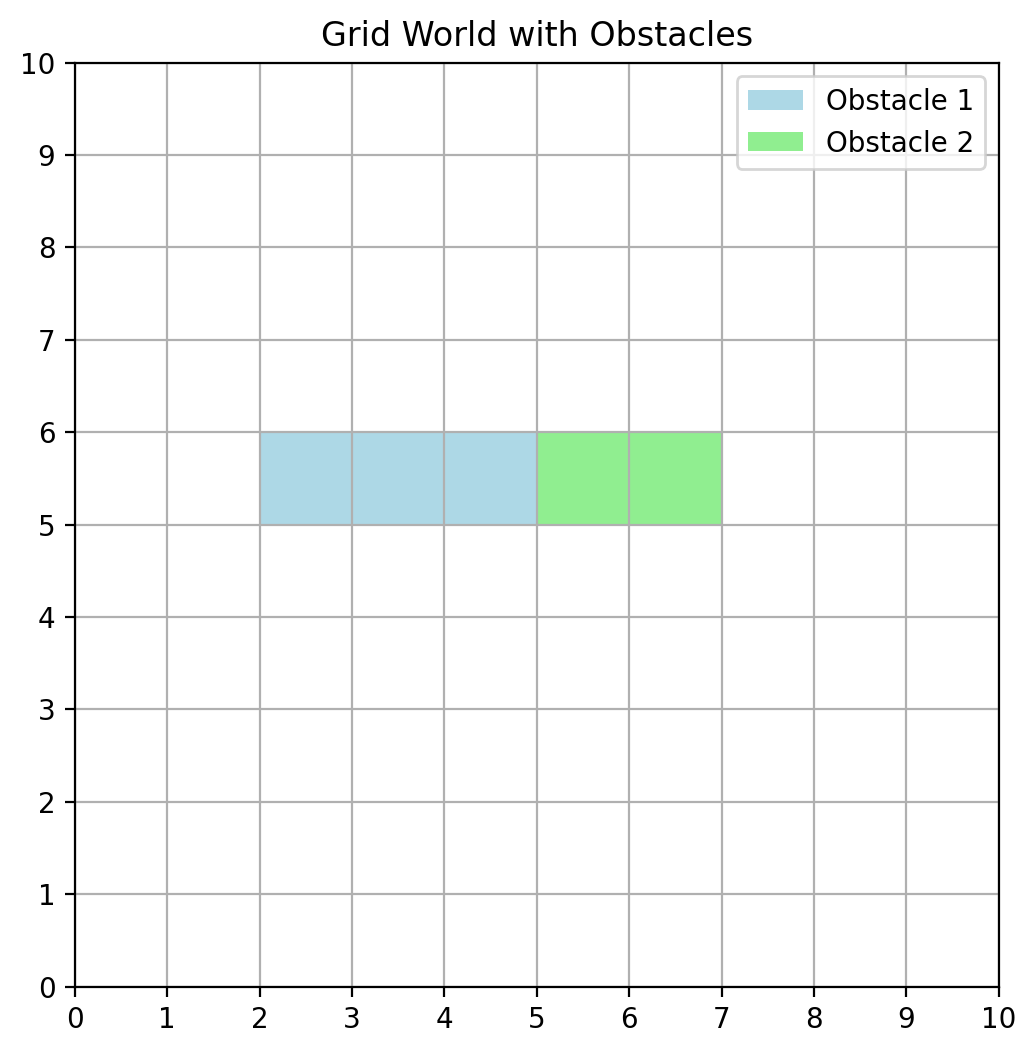
\includegraphics[width=\linewidth]{figures/world.png}
  \caption{The grid world.}
\end{subfigure}\hfill
\begin{subfigure}[t]{0.42\linewidth}
  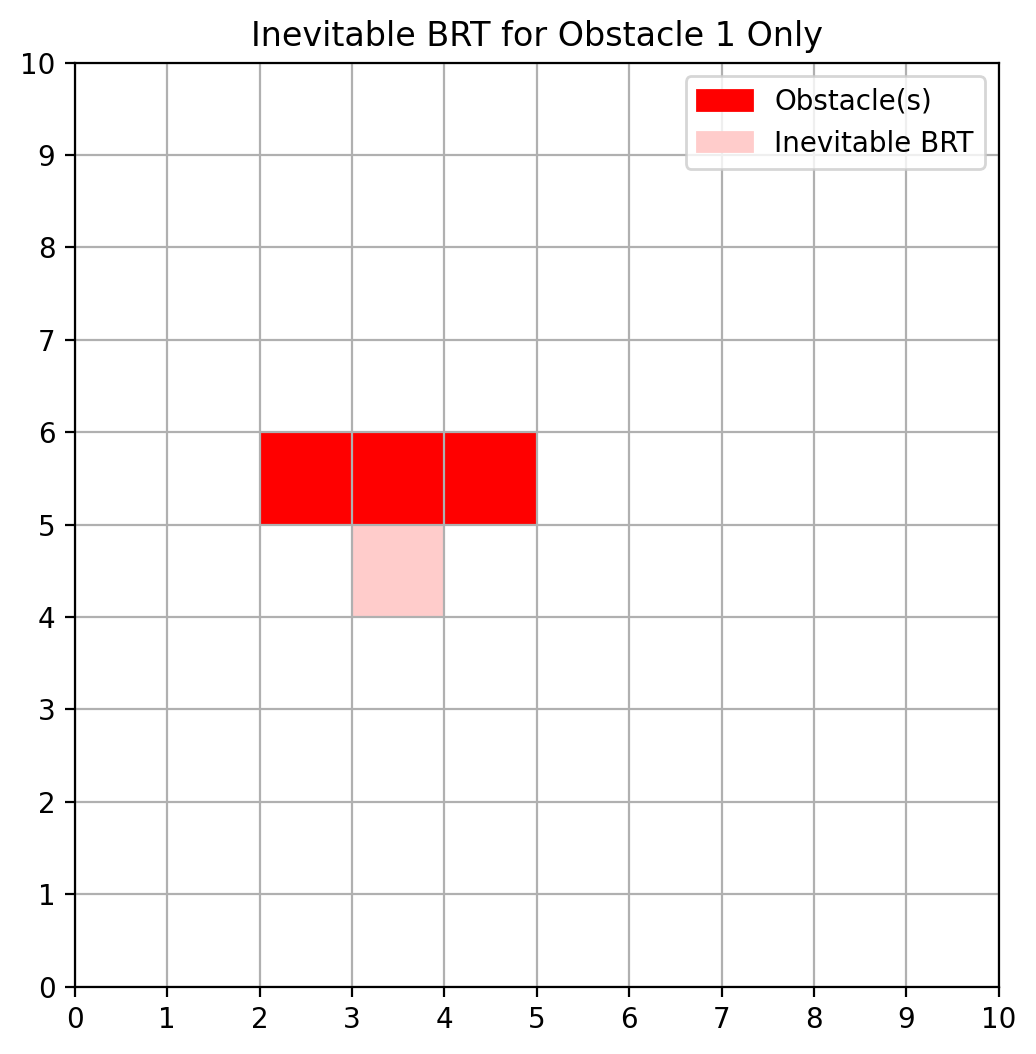
\includegraphics[width=\linewidth]{figures/brt_obstacle1.png}
  \caption{Obstacle 1 only.}
\end{subfigure}\\[2mm]
\begin{subfigure}[t]{0.42\linewidth}
  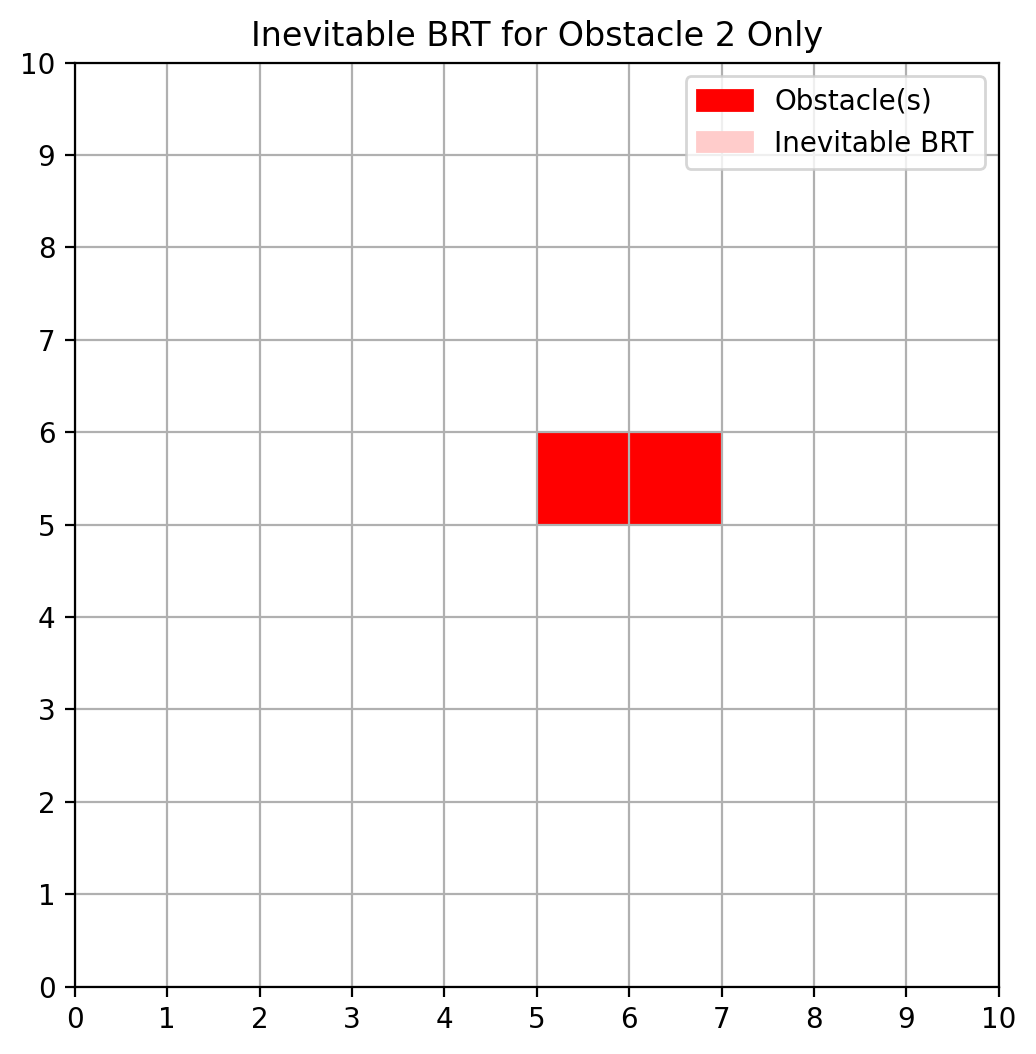
\includegraphics[width=\linewidth]{figures/brt_obstacle2.png}
  \caption{Obstacle 2 only.}
\end{subfigure}\hfill
\begin{subfigure}[t]{0.42\linewidth}
  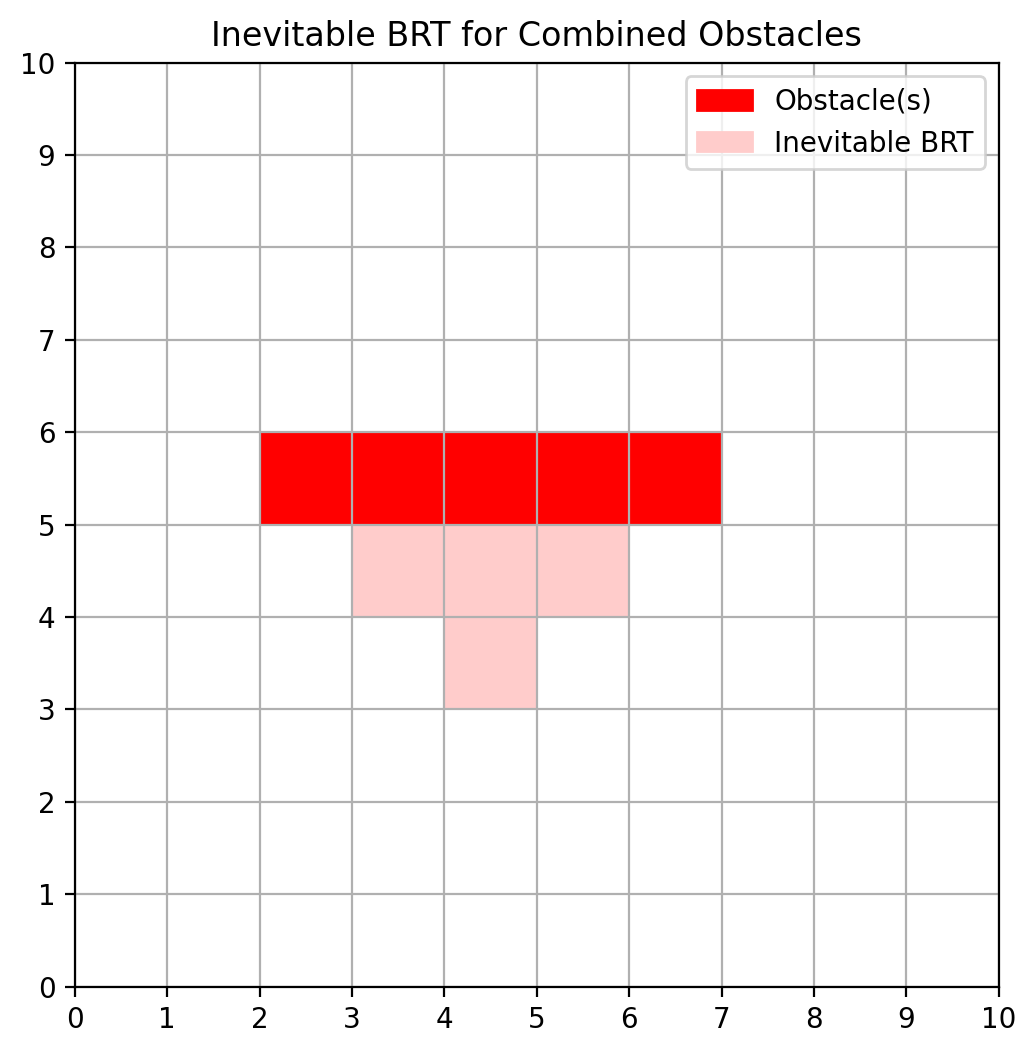
\includegraphics[width=\linewidth]{figures/brt_combined.png}
  \caption{Both obstacles.}
\end{subfigure}
\caption{Inevitable backward-reachable tubes (light red) of the obstacle sets (red).}
\label{fig:brt}
\end{figure}

\subsection*{Discussion}

\paragraph{Why the tubes look the way they do.}
The robot cannot stop or slow down, so a cell $d$ rows below the obstacle row will land on that row
after exactly $d$ steps, at a column anywhere in $\{x-d,\dots,x+d\}$ (any integer in that range is
attainable by an appropriate control sequence). Collision is inevitable if and only if
\emph{every} one of those landing columns is occupied, i.e.\ $\{x-d,\dots,x+d\}\subseteq$ obstacle
columns. For a contiguous obstacle of width $w$ this means $2d\le w-1$, so the tube is an inverted
triangle (a cone with unit slope) of height $\lfloor (w-1)/2\rfloor$ below the obstacle's centre:
height $1$ for the width-3 obstacle, height $0$ for the width-2 obstacle, and height $2$ for the
combined width-5 obstacle. This is exactly what the code produces, and it matches intuition: since
the robot's lateral speed equals its forward speed, it can escape any obstacle whose half-width is
smaller than its current distance to the obstacle row, so the doomed region hugs the obstacle
tightly. Everything above the obstacle row and everything in the rows below it that is outside the
cone is safe. Note that the width-2 obstacle alone has an empty tube beyond itself: from $(5,4)$ or
$(6,4)$ the robot can always step to a free neighbouring column.

\paragraph{Combined obstacles versus the union of the individual tubes.}
The union of the two individual tubes adds only $(3,4)$ to the obstacle cells, whereas the tube of
the combined failure set adds $(3,4)$, $(4,4)$, $(5,4)$ and $(4,3)$ (Figure~\ref{fig:union}). The
combined tube \emph{strictly contains} the union. The extra cells are states from which every escape
from one obstacle lands in the other: from $(4,4)$, steering left or going straight hits obstacle~1
while steering right hits obstacle~2, and from $(4,3)$ all three successors are among these doomed
cells. This is the discrete version of Problem~1.2(c): a state can be safe with respect to
$\failure_1$ and safe with respect to $\failure_2$ using two \emph{different} controllers, yet unsafe
with respect to $\failure_1\cup\failure_2$, i.e.\
$\safeset(\failure_1\cup\failure_2)\subsetneq\safeset(\failure_1)\cap\safeset(\failure_2)$ and,
equivalently, $\inevitable{\backward{\reach}}(\failure_1\cup\failure_2)\supsetneq
\inevitable{\backward{\reach}}(\failure_1)\cup\inevitable{\backward{\reach}}(\failure_2)$. The
practical lesson is that safety analysis must be carried out on the \emph{full} failure set;
per-obstacle tubes cannot simply be unioned, and a ``harmless'' obstacle (obstacle~2 alone traps
nothing) can enlarge the unsafe region substantially once it sits next to another one. The boundary
of the tube is also where a least-restrictive safety filter would have to intervene: from $(3,3)$
the only safe action is $\ctrl=-1$, so the filter must override $\ctrl\in\{0,+1\}$ there, while it
can leave the controller free anywhere outside the tube.

\begin{figure}[h]
\centering
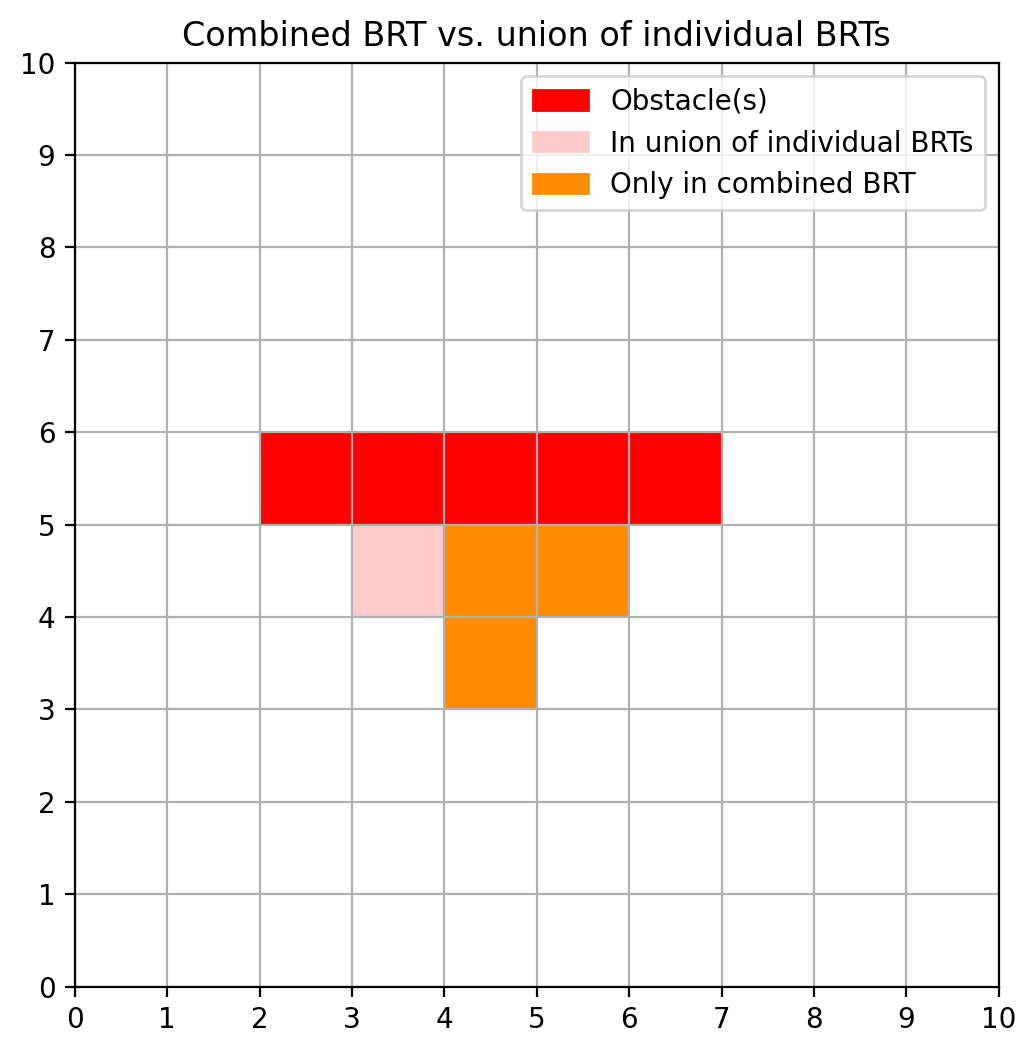
\includegraphics[width=0.42\linewidth]{figures/brt_union_vs_combined.png}
\caption{The tube of the combined failure set. Light red cells also belong to the union of the two
individual tubes; orange cells belong only to the combined tube.}
\label{fig:union}
\end{figure}

\paragraph{Effect of the forward-to-lateral speed ratio.}
The shape of the tube is set by the ratio of lateral to forward speed. If the robot advanced $v$
rows per step while still shifting by at most one column (equivalently, it could steer only once
every $v$ rows), then from $d$ rows away it could only reach columns within $\pm d/v$ of its current
one, and the trapping condition becomes $2d/v\le w-1$: the cone becomes steeper and its height grows
to about $v(w-1)/2$, so the inevitable tube \emph{grows}. A faster robot has fewer steps in which to
swerve, and in the limit of very fast forward motion every cell in the obstacle's ``shadow''
directly below it becomes doomed. Conversely, more lateral authority ($\ctrl\in\{-k,\dots,k\}$)
flattens the cone to height $\lfloor (w-1)/(2k)\rfloor$; with $k=2$ the combined tube would shrink to
the obstacles plus the single cell $(4,4)$, and obstacle~1's tube would shrink to the obstacle itself.
(In the literal discrete model a speed of $v=2$ rows per step also introduces a parity effect: a
robot starting on an even row would hop over the single obstacle row entirely, since grazing is
allowed. The statement above should therefore be read in the fine-grid or continuous-time limit,
where the obstacle has finite thickness.)
.
% Paths (figures/, *.py) are relative to the directory of hw.tex.

%===============================================================================
\section*{Problem 3: Backward Reachable Set -- Programming}
%===============================================================================

\subsection*{Implementation}

The robot advances one row per step and can shift by at most one column,
$(x_{\tvar+1},y_{\tvar+1})=(x_\tvar+\ctrl_\tvar,\,y_\tvar+1)$ with $\ctrl_\tvar\in\{-1,0,1\}$;
landing on an obstacle cell is a failure. \lstinline{get_successors} returns the cells reachable in
one step (moves that would leave the grid are treated as inadmissible; for the obstacle layout in
this problem the tube never touches the side walls, so this choice does not affect the results).
\lstinline{calculate_inevitable_brt} computes the inevitable BRT of the failure set $\failure$ by
the fixed-point iteration
\[
\inevitable{\backward{\reach}}_{0}=\failure,\qquad
\inevitable{\backward{\reach}}_{k+1}=\inevitable{\backward{\reach}}_{k}\ \cup\
\bigl\{\state:\ \dyn(\state,\ctrl)\in\inevitable{\backward{\reach}}_{k}\ \text{for \emph{all}}\ \ctrl\in\{-1,0,1\}\bigr\},
\]
i.e.\ a cell is added when every admissible control leads into the current set (no escape route),
and the iteration stops when a sweep adds nothing. Because $y$ increases by one every step, only the
rows below the highest obstacle row can ever collide, and the loop converges after at most that many
sweeps. The complement of the resulting set is the (all-time) safe set $\safeset(\failure)$; this is
the discrete-time, finite-state counterpart of the HJ reachability formulation
in~\cite{bansal2017hamilton}.

\lstinputlisting[language=Python]{get_successors.py}
\lstinputlisting[language=Python]{calculate_inevitable_brt.py}

\subsection*{Results}

\noindent\begin{minipage}{\linewidth}
Figure~\ref{fig:brt} shows the grid world and the three inevitable BRTs produced by the notebook.
With obstacle~1 occupying columns $\{2,3,4\}$ of row~5 and obstacle~2 occupying columns $\{5,6\}$:
\begin{center}
\begin{tabular}{ll}
\hline
failure set & inevitable BRT minus the obstacle cells \\
\hline
obstacle 1 (width 3) & $\{(3,4)\}$ \\
obstacle 2 (width 2) & $\emptyset$ \\
both obstacles (width 5) & $\{(3,4),(4,4),(5,4),(4,3)\}$ \\
\hline
\end{tabular}
\end{center}
\end{minipage}

\begin{figure}[h]
\centering
\begin{subfigure}[t]{0.42\linewidth}
  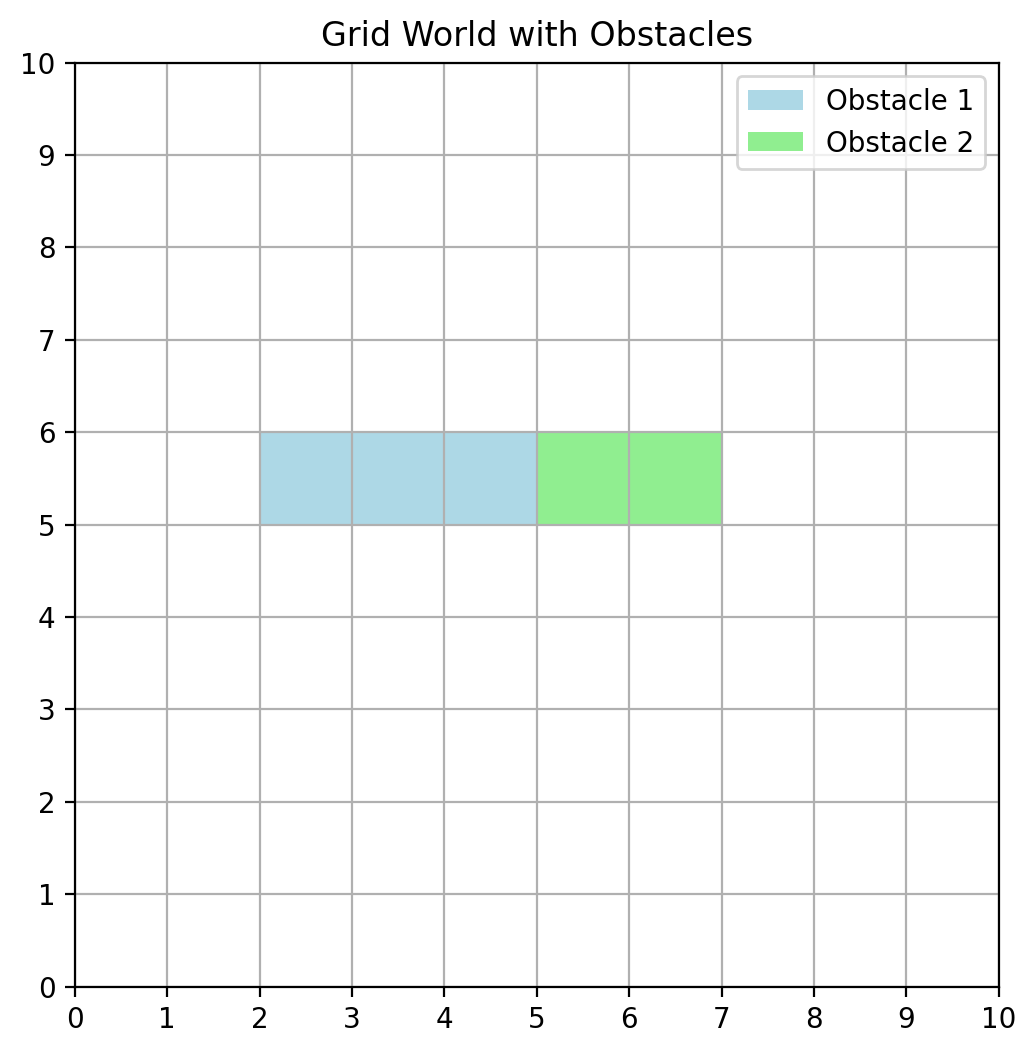
\includegraphics[width=\linewidth]{figures/world.png}
  \caption{The grid world.}
\end{subfigure}\hfill
\begin{subfigure}[t]{0.42\linewidth}
  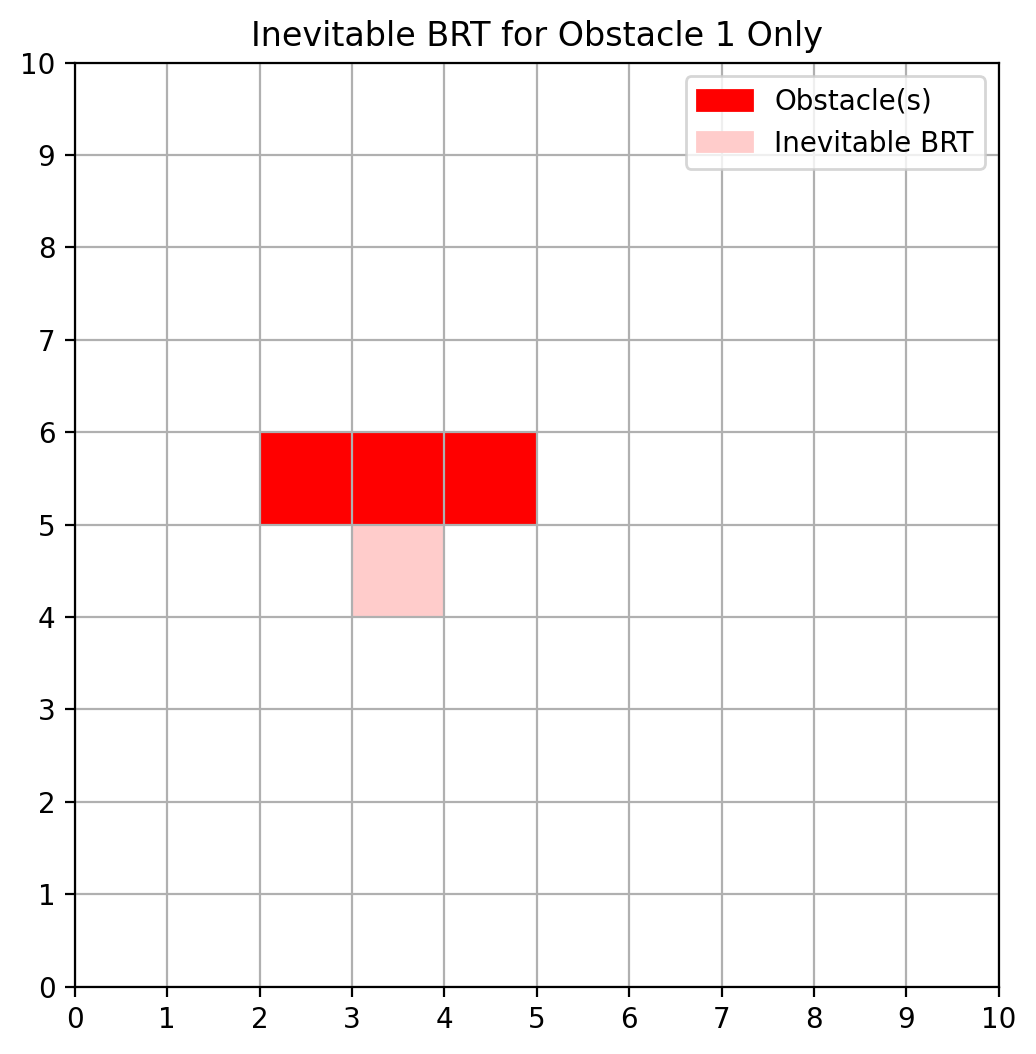
\includegraphics[width=\linewidth]{figures/brt_obstacle1.png}
  \caption{Obstacle 1 only.}
\end{subfigure}\\[2mm]
\begin{subfigure}[t]{0.42\linewidth}
  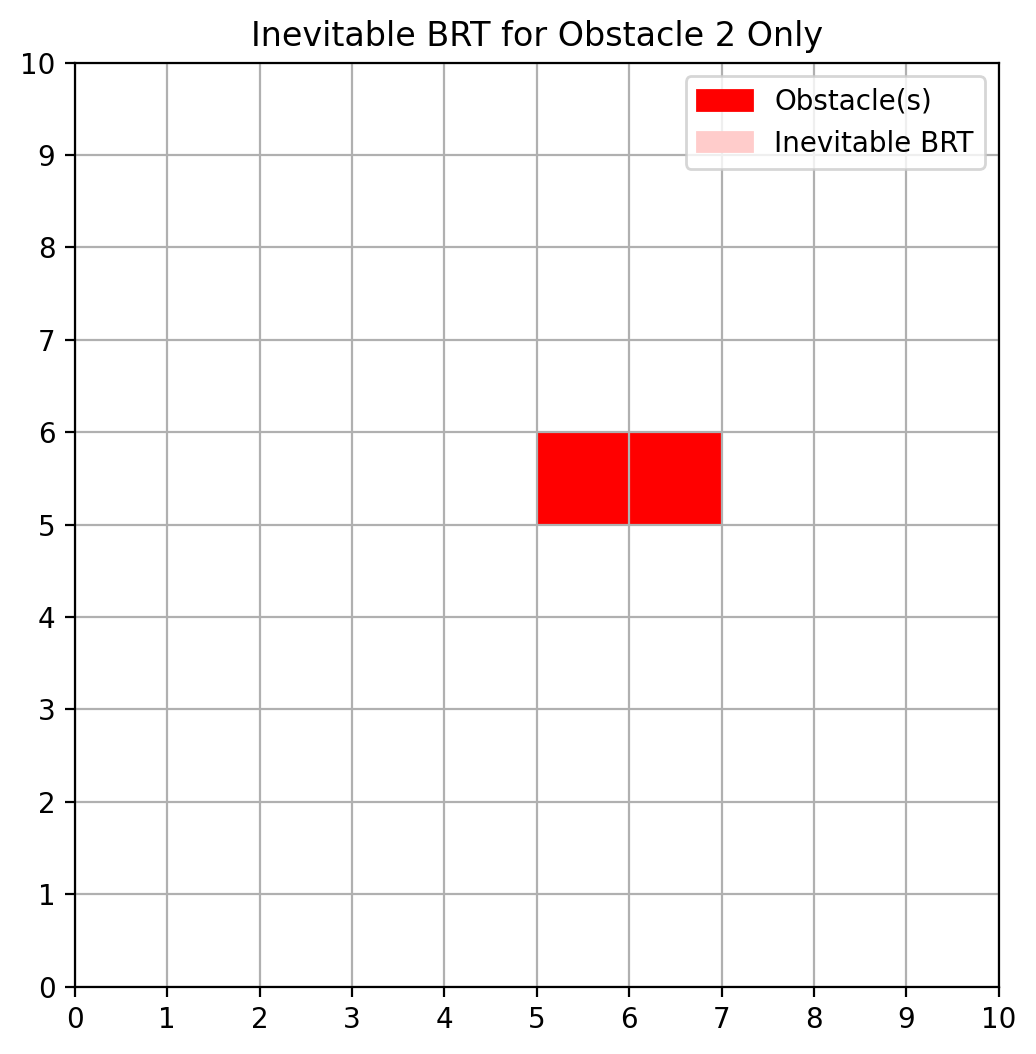
\includegraphics[width=\linewidth]{figures/brt_obstacle2.png}
  \caption{Obstacle 2 only.}
\end{subfigure}\hfill
\begin{subfigure}[t]{0.42\linewidth}
  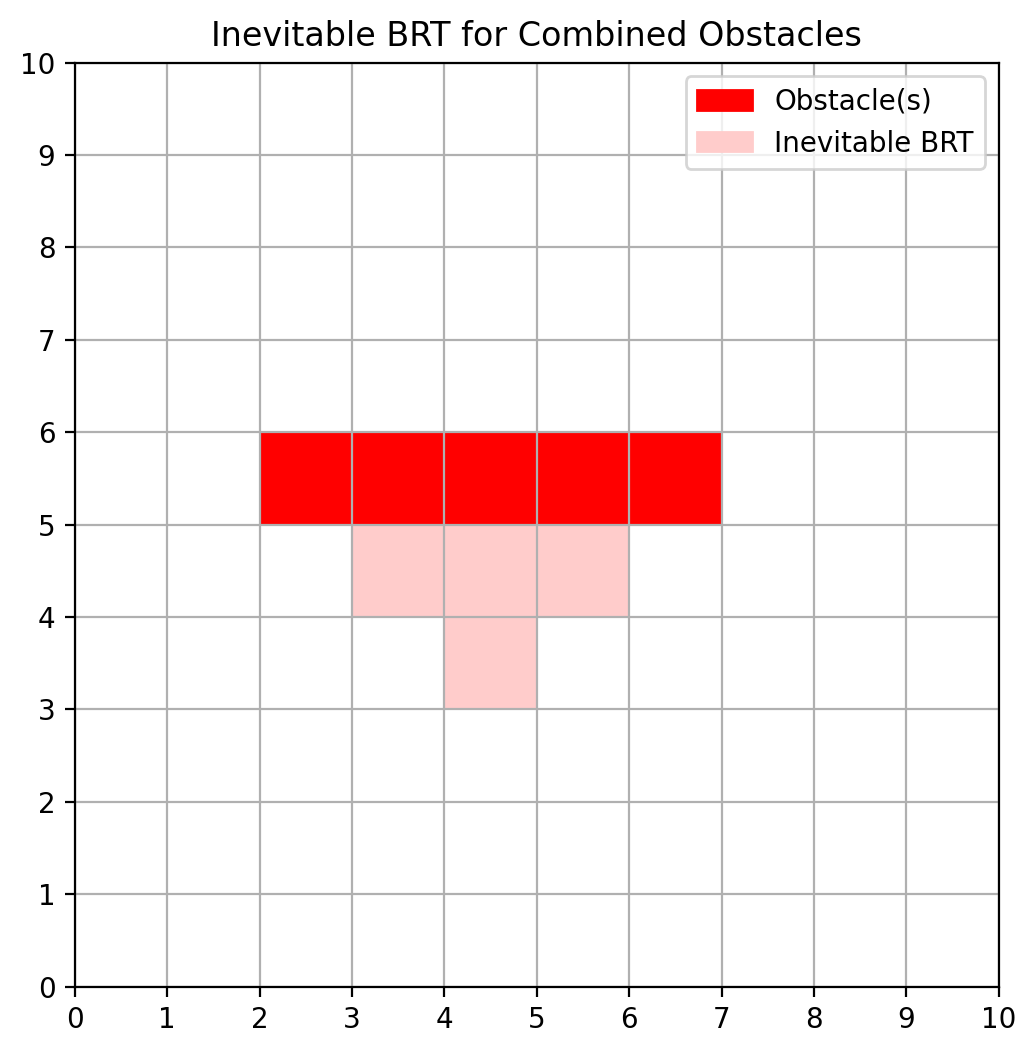
\includegraphics[width=\linewidth]{figures/brt_combined.png}
  \caption{Both obstacles.}
\end{subfigure}
\caption{Inevitable backward-reachable tubes (light red) of the obstacle sets (red).}
\label{fig:brt}
\end{figure}

\subsection*{Discussion}

\paragraph{Why the tubes look the way they do.}
The robot cannot stop or slow down, so a cell $d$ rows below the obstacle row will land on that row
after exactly $d$ steps, at a column anywhere in $\{x-d,\dots,x+d\}$ (any integer in that range is
attainable by an appropriate control sequence). Collision is inevitable if and only if
\emph{every} one of those landing columns is occupied, i.e.\ $\{x-d,\dots,x+d\}\subseteq$ obstacle
columns. For a contiguous obstacle of width $w$ this means $2d\le w-1$, so the tube is an inverted
triangle (a cone with unit slope) of height $\lfloor (w-1)/2\rfloor$ below the obstacle's centre:
height $1$ for the width-3 obstacle, height $0$ for the width-2 obstacle, and height $2$ for the
combined width-5 obstacle. This is exactly what the code produces, and it matches intuition: since
the robot's lateral speed equals its forward speed, it can escape any obstacle whose half-width is
smaller than its current distance to the obstacle row, so the doomed region hugs the obstacle
tightly. Everything above the obstacle row and everything in the rows below it that is outside the
cone is safe. Note that the width-2 obstacle alone has an empty tube beyond itself: from $(5,4)$ or
$(6,4)$ the robot can always step to a free neighbouring column.

\paragraph{Combined obstacles versus the union of the individual tubes.}
The union of the two individual tubes adds only $(3,4)$ to the obstacle cells, whereas the tube of
the combined failure set adds $(3,4)$, $(4,4)$, $(5,4)$ and $(4,3)$ (Figure~\ref{fig:union}). The
combined tube \emph{strictly contains} the union. The extra cells are states from which every escape
from one obstacle lands in the other: from $(4,4)$, steering left or going straight hits obstacle~1
while steering right hits obstacle~2, and from $(4,3)$ all three successors are among these doomed
cells. This is the discrete version of Problem~1.2(c): a state can be safe with respect to
$\failure_1$ and safe with respect to $\failure_2$ using two \emph{different} controllers, yet unsafe
with respect to $\failure_1\cup\failure_2$, i.e.\
$\safeset(\failure_1\cup\failure_2)\subsetneq\safeset(\failure_1)\cap\safeset(\failure_2)$ and,
equivalently, $\inevitable{\backward{\reach}}(\failure_1\cup\failure_2)\supsetneq
\inevitable{\backward{\reach}}(\failure_1)\cup\inevitable{\backward{\reach}}(\failure_2)$. The
practical lesson is that safety analysis must be carried out on the \emph{full} failure set;
per-obstacle tubes cannot simply be unioned, and a ``harmless'' obstacle (obstacle~2 alone traps
nothing) can enlarge the unsafe region substantially once it sits next to another one. The boundary
of the tube is also where a least-restrictive safety filter would have to intervene: from $(3,3)$
the only safe action is $\ctrl=-1$, so the filter must override $\ctrl\in\{0,+1\}$ there, while it
can leave the controller free anywhere outside the tube.

\begin{figure}[h]
\centering
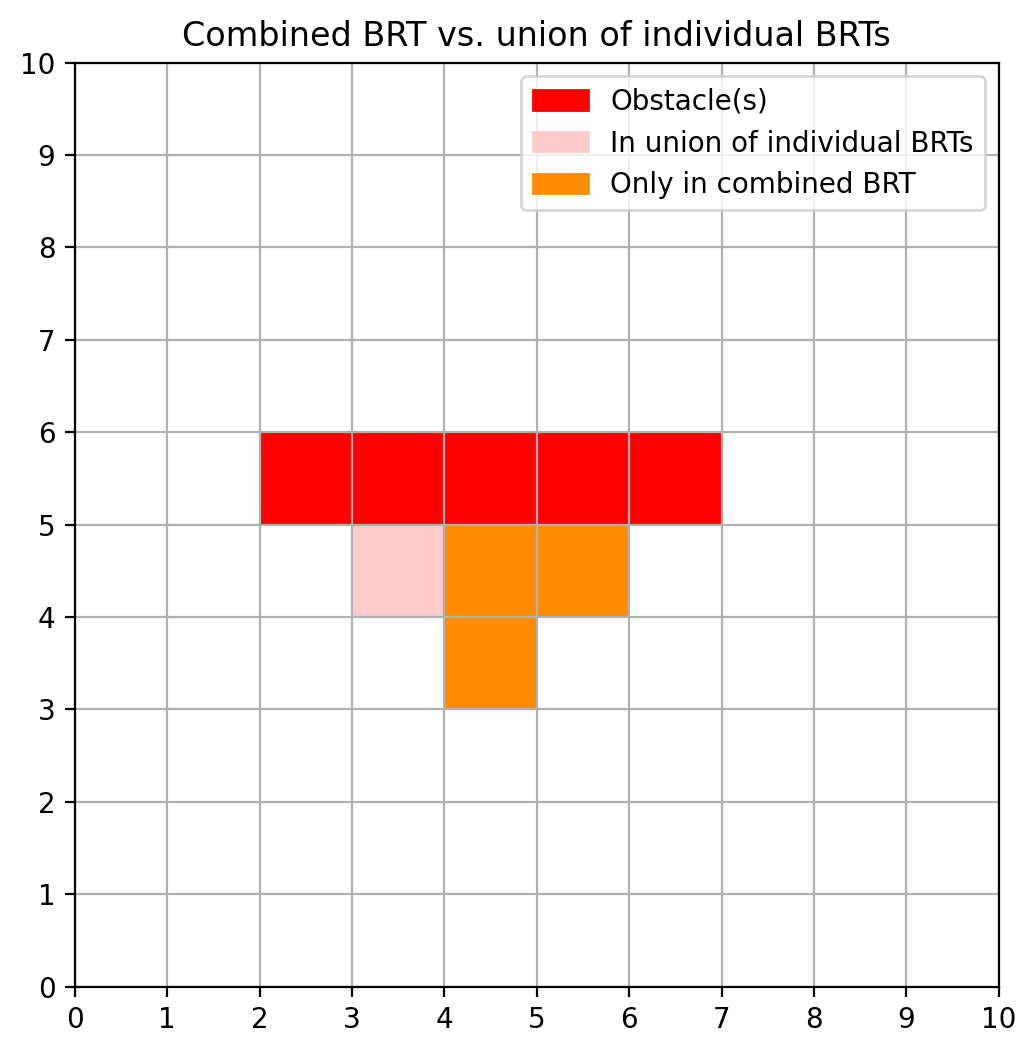
\includegraphics[width=0.42\linewidth]{figures/brt_union_vs_combined.png}
\caption{The tube of the combined failure set. Light red cells also belong to the union of the two
individual tubes; orange cells belong only to the combined tube.}
\label{fig:union}
\end{figure}

\paragraph{Effect of the forward-to-lateral speed ratio.}
The shape of the tube is set by the ratio of lateral to forward speed. If the robot advanced $v$
rows per step while still shifting by at most one column (equivalently, it could steer only once
every $v$ rows), then from $d$ rows away it could only reach columns within $\pm d/v$ of its current
one, and the trapping condition becomes $2d/v\le w-1$: the cone becomes steeper and its height grows
to about $v(w-1)/2$, so the inevitable tube \emph{grows}. A faster robot has fewer steps in which to
swerve, and in the limit of very fast forward motion every cell in the obstacle's ``shadow''
directly below it becomes doomed. Conversely, more lateral authority ($\ctrl\in\{-k,\dots,k\}$)
flattens the cone to height $\lfloor (w-1)/(2k)\rfloor$; with $k=2$ the combined tube would shrink to
the obstacles plus the single cell $(4,4)$, and obstacle~1's tube would shrink to the obstacle itself.
(In the literal discrete model a speed of $v=2$ rows per step also introduces a parity effect: a
robot starting on an even row would hop over the single obstacle row entirely, since grazing is
allowed. The statement above should therefore be read in the fine-grid or continuous-time limit,
where the obstacle has finite thickness.)
